\documentclass[11pt,a4paper]{article}
\usepackage[T1]{fontenc}
\usepackage{lmodern}
\usepackage[utf8]{inputenc}
\usepackage[margin=1in]{geometry}
\usepackage{amsmath,amssymb,bm,booktabs}
\usepackage{tikz,pgfplots}
\usetikzlibrary{arrows.meta,positioning,calc}
\pgfplotsset{compat=1.18}
\usepackage{microtype}
\usepackage[colorlinks=true,linkcolor=blue,urlcolor=blue,citecolor=blue]{hyperref}
\usepackage[most]{tcolorbox}
\newtcolorbox{keypoint}{breakable,colback=blue!3,colframe=blue!55!black,title=Interpretation,fonttitle=\bfseries}
\newcommand{\vect}[1]{\boldsymbol{#1}}
\title{Interpretation of Inverse Dynamics:\\Understanding the Fundamental Limitations}
\author{Dieter Olson}
\date{Revised September 8, 2026}
\begin{document}
\maketitle
\begin{abstract}
A golf-club torque plot can be mechanically correct and still be given an unsupported physiological interpretation. The remedy is to separate four questions: what net hand wrench follows from measured motion and known external loads; how that wrench is represented at a chosen point; which contact distributions can produce it; and what those distributions imply about muscle activity, work and perceived effort. This article derives the relevant balances, gives explicit counterexamples and distinguishes control-affine bookkeeping from an experiment in relaxation. Aerodynamic loading provides a worked example of model error: an omitted wrench changes the inferred hand wrench, but the correction has no universal sign or percentage. The same reasoning applies to bimanual humanoid manipulation, where contact redundancy, closed-chain dynamics and actuator allocation must be treated together.
\end{abstract}
\tableofcontents

\section{What Inverse Dynamics Identifies}
\subsection{Start With a System Boundary}
Inverse dynamics infers loads consistent with motion under a declared mechanical model. It does not bypass that model, and it does not infer intent directly. For the isolated club, the hands are external contacts. For the combined golfer--club system, those same contacts are internal interfaces, while ground, gravity, air and ball contact remain external. A force omitted at one boundary cannot be explained away by changing its name at another.

For the first derivation, approximate the club as rigid, take uniform gravity and work in a fixed right-handed inertial frame. Let $C$ denote the center of mass, $m$ the mass, $I_C$ the inertia tensor about $C$ expressed in that frame, and $\vect\omega$ and $\vect\alpha$ the angular velocity and acceleration in that frame. The total external balances are
\begin{align}
\vect F_{\rm total}&=m\vect a_C,\label{eq:force_balance}\\
\vect M_{{\rm total},C}&=I_C\vect\alpha+
\vect\omega\times(I_C\vect\omega).\label{eq:moment_balance}
\end{align}
The rotational expression follows by differentiating angular momentum; the gyroscopic term accounts for the changing orientation of the inertia tensor. It is not a separate hand torque. An equivalent body-frame Euler equation can be used, provided every vector, derivative and tensor convention is consistent \cite{lynch,featherstone}.

Let $\vect F_a,\vect M_{a,C}$ collect specified non-hand, non-gravitational loads, including aerodynamic loads and, when relevant, ball or turf contact. Then
\begin{align}
\vect F_h&=m\vect a_C-m\vect g-\vect F_a,\label{eq:handforce}\\
\vect M_{h,C}&=I_C\vect\alpha+
\vect\omega\times(I_C\vect\omega)-\vect M_{a,C}.\label{eq:handmoment}
\end{align}
Uniform gravity has zero moment about $C$. If collision loading is unknown, club motion alone does not separate its wrench from the hand wrench. A preimpact smooth-motion model should not be extended through collision without resolving that additional load and the relevant time scale.

The result is a \emph{hand-on-club} wrench. The club-on-hand wrench has the opposite force and moment at the same point in the same frame. Reversing the action convention halfway through an argument reverses the interpretation of a torque sign.

\subsection{Transport the Recovered Wrench}
For a grip reporting point $P$, summing moments of the original forces gives
\begin{equation}
\vect M_{h,P}=\vect M_{h,C}+(\vect r_C-\vect r_P)\times\vect F_h.
\label{eq:transport}
\end{equation}
The sign is fixed by the vector from $P$ to $C$. The general change to another point $Q$ is
\begin{equation}
\vect M_{h,Q}=\vect M_{h,P}+(\vect r_P-\vect r_Q)\times\vect F_h.
\label{eq:couple_transform}
\end{equation}
The force is unchanged by a change of origin. If the axes also rotate, rotate the force and translated moment into the new basis.

This is a transformation of a wrench, not a new angular-momentum balance about a moving pivot. In particular, substituting an arbitrary accelerating grip point into $I_P\vect\alpha+\vect\omega\times I_P\vect\omega$ generally misses transport terms. Recovering the wrench about the center of mass and then using Equation~\ref{eq:transport} avoids that mistake.

\begin{keypoint}
A reporting point is a convention. Once the net wrench and geometry are known, its change of reference is determined exactly. Uncertainty enters through uncertain motion, calibration, inertial properties, external loads or point location; it does not arise merely because two correct reports use different origins.
\end{keypoint}

\subsection{What a Rigid Approximation Leaves Out}
A shaft transmits bending, torsion and axial load. When those deformations matter, the whole club does not have one angular velocity and a constant body-frame inertia tensor. Use a distributed model or segment momentum balances, including deformation and the actual contact velocities. The total linear momentum balance still holds, and the angular momentum rate about the center of mass is still meaningful, but its rigid-body expression need not be accurate.

Motion reconstruction must therefore match the inferred quantity. Tracking only the head cannot generally recover the momentum of a flexing shaft. Tracking two shaft points does not determine rotation about their line. Marker calibration, internal mass distribution and synchronization are part of the inference. The question is whether their uncertainties are small enough for the particular load or comparison, not whether a device is generically ``accurate.''

\section{A Moment Is Real, but Its Representation Is Not a Hand Strategy}
\subsection{Single Force and Force-Plus-Couple Equivalence}
A force $\vect F$ at $A$ has moment $(\vect r_A-\vect r_P)\times\vect F$ about $P$. Replacing it by the same force at $P$ and that moment as a pure couple preserves the complete rigid-body wrench. At the same rigid-body state it therefore preserves acceleration; it preserves a trajectory when the wrench histories, initial conditions and other loads are also matched.

For a concrete planar example, use $x$ to the right, $y$ upward and positive $z$ out of the page. A force $(0,4,0)$ N at $A=(0.5,0,0)$ m has a $+2$ N m moment about $P=(0,0,0)$. The equivalent representation is a $4$ N upward force at $P$ plus a $+2$ N m counterclockwise couple. It is \emph{not} equivalent to a pure $2$ N m couple alone: that couple has zero resultant force.

\begin{figure}[htbp]\centering
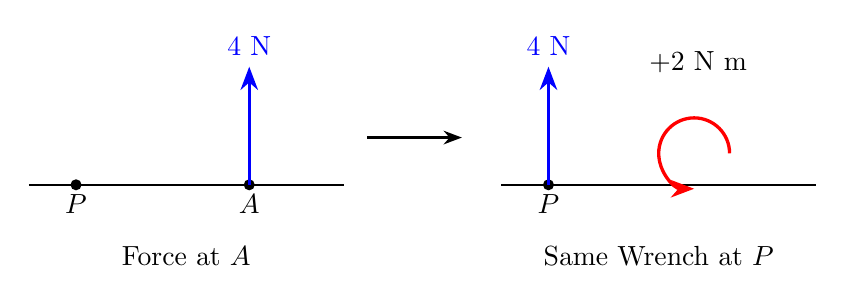
\begin{tikzpicture}[>=Stealth,scale=1]
\draw[thick] (0,0)--(4,0);\fill (0.6,0) circle(2pt);\fill (2.8,0) circle(2pt);
\node[below] at(.6,0){$P$};\node[below] at(2.8,0){$A$};
\draw[->,very thick,blue] (2.8,0)--(2.8,1.5) node[above]{$4$ N};
\node at(2,-.9){Force at $A$};
\draw[->,thick] (4.3,.6)--(5.5,.6);
\draw[thick] (6,0)--(10,0);\fill (6.6,0) circle(2pt);
\node[below] at(6.6,0){$P$};
\draw[->,very thick,blue] (6.6,0)--(6.6,1.5) node[above]{$4$ N};
\draw[->,very thick,red] (8.9,.4) arc(0:270:.45);
\node[above] at(8.5,1.3){$+2$ N m};
\node at(8,-.9){Same Wrench at $P$};
\end{tikzpicture}
\caption{One Offset Force and Its Equivalent Force-Plus-Couple Representation. The Two Diagrams Are Alternatives, Not Loads Applied Together.}
\label{fig:basic_equivalence}\end{figure}

An offset force can have a real rotational effect. Saying that its reported couple does not prove a separately applied hand couple does not mean the force has no twisting effect on the club. A hand can also apply an actual contact couple through distributed tractions. ``We only exert forces'' is therefore not a useful reason to dismiss a resultant moment: distributed forces are precisely how many physical couples are produced.

\subsection{A Free Couple Versus a Wrench's Moment Component}
A pure couple has zero resultant and is independent of origin. The moment component of a general wrench with nonzero force changes according to Equation~\ref{eq:couple_transform}. A pure couple used in one equivalent representation is a free vector; moving the \emph{force} to a different point requires changing the accompanying couple.

There is also a three-dimensional obstruction to representing every wrench by one force. For $\vect F\ne0$, the scalar $\vect F\cdot\vect M_P$ is invariant under translation. A point with zero moment exists only if that scalar is zero. One point on the central axis is
\begin{equation}
\vect r_0-\vect r_P=\frac{\vect F\times\vect M_P}{\|\vect F\|^2},
\qquad
\vect M_0=\frac{\vect F\cdot\vect M_P}{\|\vect F\|^2}\vect F.
\end{equation}
Other points on the axis differ by a displacement parallel to $\vect F$. Even when $\vect M_0=0$, the line need not intersect the grip or satisfy its contact constraints. A normal-pressure center is not automatically the application point of the complete frictional hand wrench.

\subsection{An Exact Planar Reference Sweep}
Take $\vect r_P=0$, a fixed resultant $(0,F_y,0)$ and moment $M_{P,z}$. For $Q=(s,0,0)$,
\begin{equation}
M_{Q,z}=M_{P,z}-sF_y.\label{eq:sweep}
\end{equation}
This is exactly linear for the stated fixed wrench and straight reference line. With chosen values $F_y=40$ N and $M_{P,z}=2$ N m, points at $s=-0.10,0,+0.10$ m report $6,2,-2$ N m. The zero crossing at $s=0.05$ m is a geometric fact about this wrench; it does not reveal where the fingers pressed.

\begin{figure}[htbp]\centering
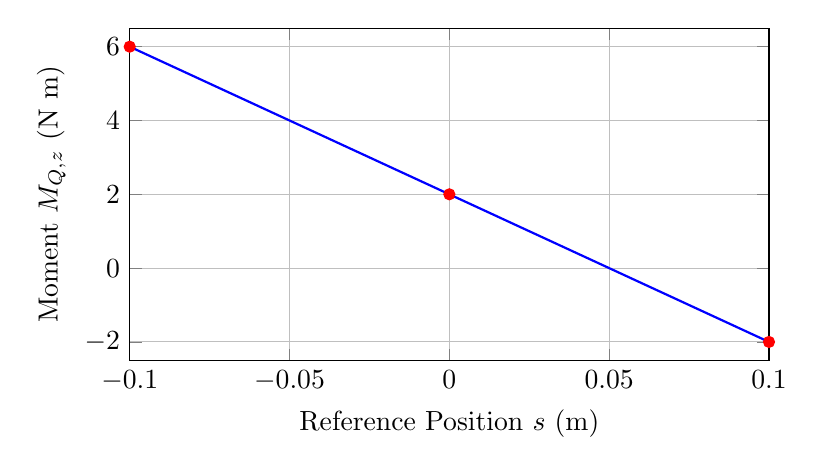
\begin{tikzpicture}\begin{axis}[width=.8\linewidth,height=5.8cm,
xlabel={Reference Position $s$ (m)},ylabel={Moment $M_{Q,z}$ (N m)},
xmin=-.1,xmax=.1,ymin=-2.5,ymax=6.5,grid=major,
xtick={-.1,-.05,0,.05,.1},scaled x ticks=false,
xticklabel style={/pgf/number format/fixed,/pgf/number format/precision=2}]
\addplot[blue,thick,domain=-.1:.1]{2-40*x};
\addplot[only marks,red] coordinates{(-.1,6)(0,2)(.1,-2)};
\end{axis}\end{tikzpicture}
\caption{Deterministic Reference Change for One Chosen Wrench. All Three Marked Values Describe the Same Loading; the Range Is Not a Confidence Interval.}
\label{fig:couple_range}\end{figure}

If positions are described relative to the center of mass by signed coordinates $d_m,d_i$, define $M_m=d_mF_y$, the moment of the force at $m$ about the center of mass. For $d_m\ne0$, Equation~\ref{eq:sweep} can be rewritten
\begin{equation}
C_i=C_m+M_m\left(1-\frac{d_i}{d_m}\right).
\end{equation}
Here $C_m,C_i$ denote wrench moments at their respective reporting points. $M_m$ is not the moment of a force about its own application point, which is zero. For fixed force and fixed reference interval, the moment range is $|F_y|\,|s_{\max}-s_{\min}|$; it does not independently grow with the distance to the center of mass. For a general three-dimensional grip, use the cross product rather than unsigned lever-arm arithmetic.

A coordinate sweep can support a useful sensitivity analysis when combined with a \emph{stated} possible contact region and contact model. It cannot by itself bound each hand's load. To ask where force might actually act is a different inverse problem from asking how to report the same wrench elsewhere.

\section{Two-Handed Contact and the Missing Allocation}
\subsection{The Grasp Map}
Let the hands contact at $\vect r_1,\vect r_2$, with forces $\vect F_i$ and local couples $\vect C_i$. About $P$,
\begin{align}
\vect F_h&=\vect F_1+\vect F_2,\\
\vect M_{h,P}&=\sum_{i=1}^2\left[(\vect r_i-\vect r_P)\times\vect F_i+\vect C_i\right].
\end{align}
Stack the contact loads in $\lambda$ and use force-first wrench ordering
$w_h=(\vect F_h,\vect M_{h,P})$. These equations define a linear grasp map
$w_h=\mathcal G(q)\lambda$ at a fixed configuration. With two arbitrary six-component hand wrenches, there are twelve unknown components and at most six independent resultant equations.

For a consistent wrench, one algebraic family is
\begin{equation}
\lambda=\mathcal G^+w_h+n,\qquad n\in\ker\mathcal G.
\end{equation}
A pseudoinverse selects a particular solution under a metric; it does not measure contact allocation. Mixing forces and moments in an unscaled Euclidean norm also introduces an arbitrary length scale. State the metric, friction, contact-area, compression and torque limits before assigning physical meaning to an optimized solution.

\subsection{An Invisible Load Pair That Really Is Invisible}
Set both local couples to zero and let
$\vect e=(\vect r_2-\vect r_1)/\|\vect r_2-\vect r_1\|$ for distinct points.
The changes
\begin{equation}
\delta\vect F_1=k\vect e,\qquad\delta\vect F_2=-k\vect e
\end{equation}
leave the resultant zero and add moment
$(\vect r_1-\vect r_2)\times k\vect e=0$.
Thus a one-parameter family of contact forces has the same club wrench. Actual allowable $k$ depends on contact feasibility. Equal-and-opposite \emph{transverse} forces, by contrast, generally form a nonzero couple and are visible in the club's moment balance.

\begin{figure}[htbp]\centering
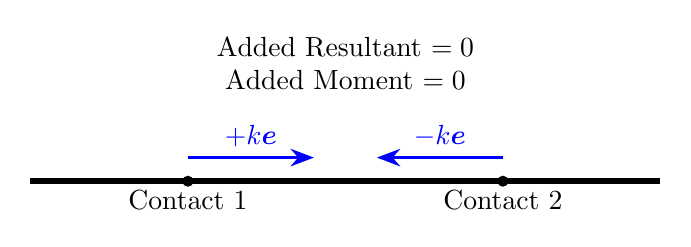
\begin{tikzpicture}[>=Stealth]
\draw[line width=2pt] (0,0)--(8,0);
\fill (2,0) circle(2pt);\fill (6,0) circle(2pt);
\node[below] at(2,0){Contact 1};\node[below] at(6,0){Contact 2};
\draw[->,very thick,blue] (2,.3)--(3.6,.3) node[midway,above]{$+k\vect e$};
\draw[->,very thick,blue] (6,.3)--(4.4,.3) node[midway,above]{$-k\vect e$};
\node[align=center] at(4,1.5){Added Resultant $=0$\\Added Moment $=0$};
\end{tikzpicture}
\caption{Collinear Opposing Contact Loads in the Grasp-Map Null Space. These Additions Preserve Rigid Club Motion but Can Change Hand and Tissue Loads.}
\label{fig:distributed_forces}\end{figure}

For the two-point force-only model, the grasp map generically has rank five: the moment component parallel to the line between contacts is constrained by the resultant. Adding contact couples changes the model and its rank. Statements that there are always six freely assignable resultant components, or that every closed chain necessarily has the same indeterminacy, are too broad.

The closed loop is completed through the two arms and torso as well as the club. Constraint geometry and redundant actuation are related, but neither the word ``affine'' nor loop closure alone proves that any arbitrary input history can generate the same trajectory. Full measured motion can identify a unique net generalized input in a fully actuated, otherwise known model. What remains nonunique may be its decomposition into contacts, actuators or muscles.

\subsection{Preserving the Original Contact-Position Experiment}
The handwritten example also asks a different, valid question: what changes if the same force magnitudes move on the grip? At a fixed midpoint $P$, let $x$ point toward the head, $y$ upward and positive $z$ out of the page. Apply $F_{L,y}=-10$ lbf and $F_{R,y}=15$ lbf. In Case 1 their signed positions are $x_L=-2$ inches and $x_R=+1$ inch; in Case 2 they are $-1$ and $+2$ inches. Both have a $+5$ lbf resultant, but
\begin{align}
M_{P,z}^{(1)}&=(-2)(-10)+(1)(15)=35\text{ lbf in},\\
M_{P,z}^{(2)}&=(-1)(-10)+(2)(15)=40\text{ lbf in}.
\end{align}
These are approximately $3.9545$ and $4.5194$ N m, a $14.3\%$ increase relative to Case 1. The original sheet reports negative values because it uses clockwise-positive moments. Its approximate fifteen-percent comparison is a chosen example, not a measured population effect.

Here the forces physically move while the reporting point stays fixed, so the two club wrenches differ. This is not the same experiment as transporting one unchanged wrench to a new reporting point. Nor does it demonstrate two different allocations with identical inverse-dynamics output; that requires preserving both resultant force and moment, as in the collinear null-space example. Keeping these three experiments distinct preserves what the original question is trying to investigate.

\subsection{What Extra Measurements Add}
An instrumented grip can constrain hand resultants, and distributed pressure/shear measurements can constrain contact tractions. The sensor's calibration, bandwidth and perturbation of the grip matter. Ground-force measurements constrain the whole-body external wrench, but do not by themselves identify every hand force or muscle force. Full-body motion, segment inertias and additional contact information can reduce the family of admissible loads.

Electromyography is evidence about electrical activity, not a direct conversion to muscle force or conscious intent. Muscle geometry, activation dynamics, force--length/velocity behavior, tendon compliance and co-contraction need their own model and validation. A model that fits the club motion can still predict implausible or unmeasured tissue loads. That mismatch is a reason to revise the model, not to rename its residual ``effort.''

\section{Control-Affine Dynamics Without Double Counting}
\subsection{One Mechanical Balance, Two Useful Arrangements}
In independent generalized coordinates, write
\begin{equation}
M(q)\ddot q+h(q,\dot q)=B(q)u+Q_{\rm ext}.
\label{eq:lagrange}
\end{equation}
The bias $h$ contains the terms placed on the left, such as velocity coupling, gravity and declared constitutive loads; $Q_{\rm ext}$ contains known external generalized loads not already included there. With positive-definite $M$, define
\begin{align}
a_d&=M^{-1}(Q_{\rm ext}-h),\\
\tau_{\rm ID}&=M\ddot q+h-Q_{\rm ext}=Bu.\label{eq:inverse_dynamics}
\end{align}
Therefore $\tau_{\rm ID}=M(\ddot q-a_d)$. Standard inverse dynamics already accounts for the declared drift terms. Subtracting another ``drift torque'' from this output would double-count them.

For $x=(q,\dot q)$, the same system is
\begin{equation}
\dot x=\underbrace{\begin{bmatrix}\dot q\\a_d\end{bmatrix}}_{f(x)}+
\underbrace{\begin{bmatrix}0\\M^{-1}B\end{bmatrix}}_{G(x)}u.
\label{eq:control_affine}
\end{equation}
Known time-dependent loads may make this $f(x,t),G(x,t)$. The first-order left side is $\dot x$, not $\ddot x$. Control-affine means linear in the selected instantaneous input at a fixed state; it does not mean linear state dynamics or superposable swing trajectories.

One can instead partition the acceleration resultant:
\begin{equation}
M\ddot q=\underbrace{(Q_{\rm ext}-h)}_{\tau_{\rm drift}}
+\underbrace{Bu}_{\tau_{\rm input}}.
\end{equation}
This equation is consistent if its left side is called the resultant. It becomes inconsistent if that left side is simultaneously called the inverse-dynamics applied torque $M\ddot q+h-Q_{\rm ext}$. Generalized loads are conjugate to their coordinates: not every component has units of torque.

\subsection{A Pendulum Check}
For a point mass $m$ at length $L$, measure angle $q$ from downward vertical. A pivot torque $u$ gives
\begin{equation}
mL^2\ddot q+mgL\sin q=u.
\end{equation}
Choose $m=1$ kg, $L=1$ m, $g=9.81$ m/s$^2$ and $q=30^\circ$. With $u=0$, acceleration is $-4.905$ rad/s$^2$; inverse dynamics returns
$-4.905+4.905=0$ N m. Holding the same configuration stationary requires $u=4.905$ N m. Moving under gravity and holding against gravity are different motions, but the same inverse equation handles both correctly.

\begin{table}[htbp]\centering
\begin{tabular}{lrrr}\toprule
Scenario & $\ddot q$ (rad/s$^2$) & $M\ddot q$ (N m) & $u_{\rm ID}$ (N m)\\\midrule
Zero Pivot Torque & $-4.905$ & $-4.905$ & $0$\\
Stationary Hold & $0$ & $0$ & $4.905$\\\bottomrule
\end{tabular}
\caption{Resultant and Applied Torque Differ Even in a One-Link Model.}
\end{table}

\subsection{Constraints Do Not Make Reactions Input-Independent}
With redundant coordinates and ideal bilateral constraints, write
\begin{align}
M\ddot q+h&=Bu+Q_{\rm ext}+A^T\lambda_c,\\
A\ddot q+\dot A\dot q&=0.
\end{align}
When $A$ has independent rows,
\begin{equation}
\lambda_c=-(AM^{-1}A^T)^{-1}
\left[AM^{-1}(Bu+Q_{\rm ext}-h)+\dot A\dot q\right].
\end{equation}
The reaction generally depends on $u$. Eliminating it modifies both the drift and the input gain. A nonzero reaction can coexist with zero actuator torque; that does not make every reaction an input-independent passive term. Ideal workless constraints are a modeling assumption, while friction, compliant contacts and anatomical tissues can carry power or store energy.

A wrist universal-joint approximation restricts rotations relative to a chosen anatomical model. Its reaction moments do not demonstrate that the golfer relaxed, and cannot be inferred merely from a diagram of two joint axes. The permitted degrees of freedom, compliances, other joints and contact conditions must be declared.

\subsection{Actuator Allocation and Model Error}
Return to the independent-coordinate balance in Equation~\ref{eq:lagrange}. If $B$ has full column rank and $\tau_{\rm ID}$ lies in its image, $u=B^+\tau_{\rm ID}$ is unique. Otherwise, redundant solutions may differ by $\ker B$, or no exact solution may exist. After eliminating constraints, apply this rank test to the reduced input map; full rank of the original redundant-coordinate $B$ alone does not resolve unknown constraint loads. Check the residual $\tau_{\rm ID}-BB^+\tau_{\rm ID}$ before interpreting an allocation. Muscle nonnegativity and other physiological restrictions can remove algebraic solutions or show that the model is infeasible.

A model that omits passive tissues estimates a net joint load containing their contribution. A model that subtracts a calibrated passive constitutive load estimates a different residual. Neither convention automatically measures voluntary motor command. An impedance estimate obtained during active contraction need not represent relaxed passive tissue.

If the actual and assumed models differ, their inverse outputs can differ too. With the same measured $q,\dot q,\ddot q$,
\begin{equation}
\widehat\tau_{\rm ID}-\tau_{\rm ID}
=(\widehat M-M)\ddot q+(\widehat h-h)
-(\widehat Q_{\rm ext}-Q_{\rm ext}).
\end{equation}
This is a model-error identity, not a proof that inverse dynamics assumes all motion is active. It shows which assumptions need sensitivity analysis.

\subsection{A Zero-Input Branch Is a Defined Intervention}
A zero-torque counterfactual starts from a specified state and sets selected inputs to zero under a specified model. For actual and zero-input states $x,x_0$ in a common local chart,
\begin{equation}
\frac{d}{dt}(x-x_0)=f(x)-f(x_0)+G(x)u.
\end{equation}
Only at a common state does the drift difference vanish. Later differences include changed geometry, velocity, shaft deformation and events. Specify the horizon, output and comparison event; do not call the difference between two trajectories an instantaneous muscle force.

Setting a modeled net torque to zero, freezing an identified impedance, removing muscle activation and asking a person to relax are different interventions. A relaxed golfer may change grip contact, posture and feedback. An ideal model can illuminate a mechanism without establishing what that experiment would feel like.

\section{Mechanical Power and Radial Loading}
\subsection{Power Survives a Consistent Reference Change}
For material points $P,Q$ of one rigid body,
$\vect v_Q=\vect v_P+\vect\omega\times(\vect r_Q-\vect r_P)$.
Together with Equation~\ref{eq:couple_transform}, this gives
\begin{equation}
\mathcal P_h=\vect F_h\cdot\vect v_P+\vect M_{h,P}\cdot\vect\omega
=\vect F_h\cdot\vect v_Q+\vect M_{h,Q}\cdot\vect\omega.
\label{eq:power}
\end{equation}
The two transport terms cancel by the scalar triple-product identity. Force power and moment power can change separately; their sum is invariant. Thus ``force-driven'' versus ``couple-driven'' energy fractions require a reporting point and are not intrinsic physiological categories.

For the $4$ N offset-force example, choose $\vect v_P=0$ and $\vect\omega=(0,0,2)$ rad/s. Then $\vect v_A=(0,1,0)$ m/s. At $A$, force power is $4$ W and moment power is zero. At $P$, force power is zero and moment power is $2\times2=4$ W. The actual energy transfer is identical.

For flexible interfaces, sum force and couple powers at their actual ports and include deformation power. A rigid reference transform does not reproduce bending work at different moving cross-sections. Even in a rigid model, total mechanical hand power does not equal muscle metabolic power or perceived effort; co-contraction and isometric force can require physiological effort while contributing little net external work.

\subsection{Centripetal Demand Is Not an Extra Force to Subtract}
For an ideal point mass on a massless rod with a fixed pivot, take $\vect e_r$ outward and $T>0$ as inward tension. The radial balance is
\begin{equation}
-T+m\vect g\cdot\vect e_r=-mL\omega^2,
\qquad T=mL\omega^2+m\vect g\cdot\vect e_r.
\end{equation}
At the bottom of a vertical circle, $T=mL\omega^2+mg$. These are actual rod/contact loads. An outward centrifugal term can be introduced in a rotating-frame balance, but it is not an additional physical interaction to subtract from measured tension in an inertial balance.

Choose $m=0.25$ kg, $L=1$ m and $\omega=30$ rad/s at the bottom. The required inward resultant is $225$ N, and tension is $227.4525$ N. Subtracting $225$ N and calling the remaining $2.4525$ N ``what the golfer feels'' is unjustified. The contact still transmits the full tension. The choice $m=0.25$ kg is an illustrative point-mass parameter, not a measured complete-club model.

\begin{figure}[htbp]\centering
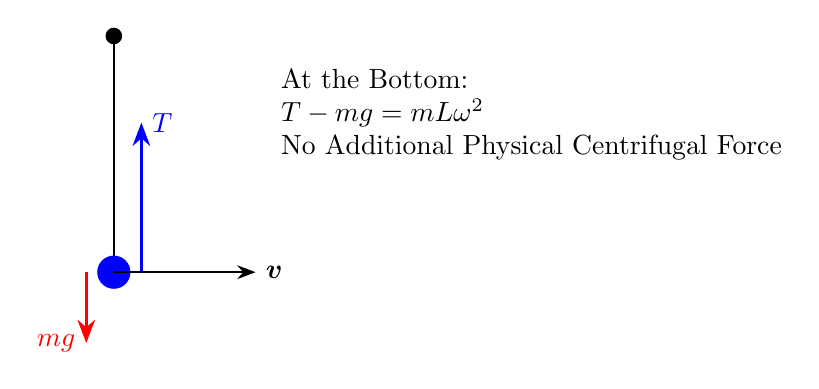
\begin{tikzpicture}[>=Stealth]
\fill (0,3) circle(3pt);\draw[thick] (0,3)--(0,0);
\fill[blue] (0,0) circle(6pt);
\draw[->,very thick,blue] (.35,0)--(.35,1.9) node[right]{$T$};
\draw[->,very thick,red] (-.35,0)--(-.35,-.9) node[left]{$mg$};
\draw[->,thick] (0,0)--(1.8,0) node[right]{$\vect v$};
\node[right,align=left] at(2,2){At the Bottom:\\$T-mg=mL\omega^2$\\No Additional Physical Centrifugal Force};
\end{tikzpicture}
\caption{Actual Loads and Radial Acceleration in a Fixed-Pivot Point-Mass Example.}
\end{figure}

The tension is perpendicular to instantaneous velocity in this example and does zero force power on the mass. Large load and zero instantaneous power can coexist. For a club with moving hands, neither the fixed-pivot radial formula nor zero grip-force power generally applies. Earlier muscle work also establishes the current speed: present redirection cannot be separated causally from the state created earlier in the swing.

\section{Aerodynamics as a Precisely Defined Omitted Wrench}
\subsection{What the Driver Study Supports}
Henrikson, Wood and Hart \cite{henrikson} tested two matched driver heads, one with crown features, in a wind tunnel and with forty players. Their near-impact tunnel condition was $96$ mph with the head at $90^\circ$ to the defined orientation scale; the plotted drag is about $9$ N versus $6.6$ N, with a reported $2.3$ N difference. Lift also changed, including its sign near that orientation. The player comparison reported about a $1$ mph mean club-speed increase; the approximately four-yard carry gain was modeled. These are driver/configuration results, not an iron-drag calibration or a universal aerodynamic center.

A seven-iron's area, geometry, orientation history and relative airflow differ. Calling it less aerodynamic does not establish its force at another speed. A quadratic drag approximation,
\begin{equation}
\vect F_D=-\tfrac12\rho C_D A\|\vect v_{\rm rel}\|\vect v_{\rm rel},
\end{equation}
requires declared density, coefficient, reference area and relative velocity. In a rotating club, distributed local airflow can matter. Lift and aerodynamic couples require additional components. Equipment geometry and orientation can change aerodynamic loading; it is not an immutable force beyond all influence.

\subsection{The Error Is the Omitted Wrench at the Same Point}
Hold the measured motion fixed. Let a superscript $0$ denote inference omitting aerodynamic loads, and let the corrected inference include them. Equations~\ref{eq:handforce}--\ref{eq:transport} give
\begin{align}
\vect F_h^0-\vect F_h&=\vect F_a,\\
\vect M_{h,P}^0-\vect M_{h,P}&=\vect M_{a,C}
 +(\vect r_C-\vect r_P)\times\vect F_a
 =\vect M_{a,P}.\label{eq:aerobias}
\end{align}
If a force acts at $D$ with intrinsic aerodynamic couple $\vect C_a$,
$\vect M_{a,P}=(\vect r_D-\vect r_P)\times\vect F_a+\vect C_a$.
Do not add the center-of-mass lever-arm correction again after the aerodynamic moment has already been expressed about $P$.

The force bias has units N and the moment bias N m, so saying one is simply ``larger'' needs a scale and an intended observable. A modest aerodynamic force can produce a large \emph{fractional} correction when the original inferred moment is small or close to cancellation. It need not dominate total hand load.

\subsection{Reconstructing the Earlier Forty-Percent Example}
The earlier draft used a $37$-inch club, a grip point $3.5$ inches from the butt, a center of mass $10$ inches from the head end and a drag application point one inch from that end. Treat those as chosen geometry, not verified measurements from a video. Use a local right-handed frame with $x$ along the shaft toward the head, $y$ transverse to the shaft and $z=x\times y$. Draw $x$ rightward and $y$ upward, so positive $z$ moment is counterclockwise. Choose the original sketch's transverse hand force to point along $-y$, and put $P$ at zero. The distances are
\begin{equation}
x_C=23.5\text{ in}=0.5969\text{ m},\qquad
x_D=32.5\text{ in}=0.8255\text{ m}.
\end{equation}
The force-to-COM separation is $9$ inches. Use $1$ lbf $=4.4482216152605$ N; pounds-force must not be inserted as a mass.

Assume the no-aerodynamics inference at $P$ is
$F_{h,y}^0=-7.5$ lbf $=-33.3616621$ N and $M_{h,P,z}^0=-18.4$ N m.
Assume zero intrinsic aerodynamic couple. Two possible signed projections of an aerodynamic force of magnitude $2$ lbf give:
\begin{table}[htbp]\centering
\begin{tabular}{lrr}\toprule
Quantity & Case A & Case B\\\midrule
$F_{a,y}$ (N) & $+8.8964$ & $-8.8964$\\
$M_{a,P,z}=x_DF_{a,y}$ (N m) & $+7.3440$ & $-7.3440$\\
$F_{h,y}=F_{h,y}^0-F_{a,y}$ (N) & $-42.2581$ & $-24.4652$\\
$M_{h,P,z}=M_{h,P,z}^0-M_{a,P,z}$ (N m) & $-25.7440$ & $-11.0560$\\\bottomrule
\end{tabular}
\caption{Two Signed Aerodynamic Scenarios for Chosen Geometry and the Same No-Aerodynamics Inference.}
\label{tab:aerocases}\end{table}

Case B reproduces the original sketch: both the hand-force magnitude in this transverse direction and the negative moment magnitude decrease, to $5.5$ lbf and $11.0560$ N m. The moment reduction is about $39.9\%$. Case A reverses the aerodynamic projection while holding the no-aerodynamics inference fixed; both magnitudes increase. Thus the original reduction is mechanically possible under its stated geometry and force direction. It is not evidence that every omitted aerodynamic load causes that reduction. Calling a force ``drag'' fixes its direction relative to airflow, not its sign in an analysis coordinate.

The retained video stills show a $7.5$ lbf user-frame force component, $-18.4$ N m user-frame alpha torque and $97.0$ mph club speed; the handwritten note says $95$ mph. The stills do not establish the complete basis transformation, iron geometry or aerodynamic load. The numerical scenario above is therefore a transparent reconstruction of the sketch, not a validated reanalysis of that swing. Its $y,z$ labels are defined here and must not be silently equated to the video's beta and alpha axes.

The same calculation can be checked about $C$. First,
$M_{h,C}^0=M_{h,P}^0-x_CF_{h,y}^0$.
Then subtract $M_{a,C}=(x_D-x_C)F_{a,y}$ and translate the corrected hand wrench back to $P$. The result is exactly Table~\ref{tab:aerocases}. This is an independent bookkeeping route, not an independent experiment.

\begin{figure}[htbp]\centering
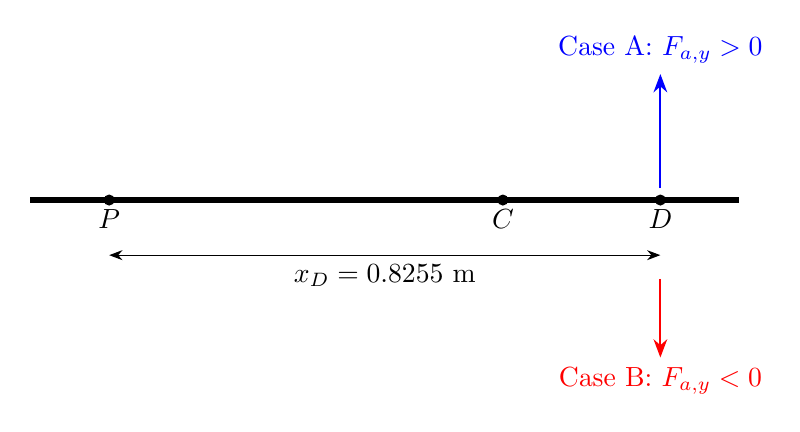
\begin{tikzpicture}[>=Stealth]
\draw[line width=2pt] (0,0)--(9,0);
\fill (1,0) circle(2pt);\fill (6,0) circle(2pt);\fill (8,0) circle(2pt);
\node[below] at(1,0){$P$};\node[below] at(6,0){$C$};\node[below] at(8,0){$D$};
\draw[<->] (1,-.7)--(8,-.7) node[midway,below]{$x_D=0.8255$ m};
\draw[->,thick,blue] (8,.15)--(8,1.6) node[above]{Case A: $F_{a,y}>0$};
\draw[->,thick,red] (8,-1)--(8,-2) node[below]{Case B: $F_{a,y}<0$};
\end{tikzpicture}
\caption{Alternative Aerodynamic Force Projections About a Fixed Grip Point. The Two Arrows Represent Separate Cases.}
\label{fig:drag_effect}\end{figure}

At a new point $Q$, the bias becomes $\vect M_{a,Q}$, while the no-drag moment also changes. A percentage computed at $P$ does not generally remain the same at $Q$; it can become ill-conditioned if the denominator crosses zero. Report signed absolute corrections and uncertainty before quoting a percentage.

\section{From Mechanical Loads to an Intertwined Swing Argument}
\subsection{Why the Links Cannot Be Read in Isolation}
Earlier muscle action changes posture, speed, contact loading and shaft deformation. Those states change the current gravity leverage, velocity coupling and input gain. The grip transmits a wrench to a flexible shaft; the shaft and head state shape the collision; the collision sets the initial ball state. A launch-monitor result constrains the end of this chain but does not uniquely recover its internal load history.

A negative component labelled ``alpha torque'' is meaningful only after defining its origin, basis, axis, action convention and whether it is a wrench projection or generalized torque. An axis tied to a moving frame has its own kinematics; its coordinate rate need not equal an angular-velocity component. A negative moment component does not alone establish negative total power, an intentional braking action, an individual hand's role or an undesirable technique.

A useful mechanism question is whether a hand-path change redistributes energy under matched initial state and work, or instead increases speed by requiring more work. Those possibilities can coexist, but they answer different questions. A large normal force, an angular-speed peak sequence or similarity to a zero-input trajectory does not settle the energy balance. Compute complete power and work, track stored elastic energy and state what intervention is feasible.

\subsection{A Layered Evidence Plan}
\begin{enumerate}
\item Define the outcome: a net hand wrench, an individual contact load, club speed, transferred work, muscle force or perceived effort. Specify the time or event.
\item Define the system boundary and convention: body segments, flexible coordinates, reporting point, frame, signs, known external loads and passive-force treatment.
\item Recover motion with an uncertainty model. Report differentiation and filtering, inertial-property uncertainty, sensor bandwidth, clock alignment and event definition.
\item Verify mechanical consistency: center-of-mass and transported moment balances, forward/inverse round trips, zero-input analytic limits, contact feasibility and power invariance.
\item Test identification separately from computation. Examine grasp-map and actuator-map ranks, admissible null-space loads and sensitivity to alternative contact or tissue models.
\item Validate against independent measurements under the intended conditions. Agreement between two rearrangements of one model tests consistency; agreement with a calibrated independent sensor addresses a different evidentiary question.
\item Test the coaching or physiological claim with the relevant intervention and measurements. Mechanical possibility is a hypothesis; performance, sensation and tissue consequences require their own evidence.
\end{enumerate}

\subsection{Uncertainty and Practical Falsifiers}
A high sample rate alone does not guarantee an accurate inverse load. Position noise is amplified by differentiation, while smoothing changes peaks and timing. The appropriate bandwidth for a preimpact swing envelope differs from that for ball contact or shaft vibration. Specify the quantity whose error matters and demonstrate sufficient temporal and spatial resolution.

For a differentiable estimate $y=\Phi(z)$, a local covariance approximation is
$\Sigma_y\approx J\Sigma_zJ^T$, with $J=D\Phi$ and all correlated inputs included. A contact-mode change or poorly localized impact event may need explicit scenario propagation rather than that local linearization. Changing a filtering cutoff, point calibration or plausible inertia can reveal whether a claimed torque-sign reversal is robust.

Concrete falsifiers include an inferred wrench outside independent sensor uncertainty, a contact allocation violating friction or compression limits, or an energy balance that fails to close within measurement and model error. A conclusion whose sign reverses under plausible aerodynamic assumptions is not ready to become a universal coaching instruction. Report the unresolved dependence and identify the measurement that would reduce it.

\section{What a Defensible Conclusion Looks Like}
Inverse dynamics can estimate net mechanical loads under a declared model. It does not inherently confuse drift with actuation, and a change of reference does not make its result fictional. The interpretive limits arise when a net wrench is treated as a unique contact pattern, a model input as a muscle command, or a mechanical power as a sensation.

The constructive route is to retain what each layer identifies and expose what it leaves open. Wrench transformations connect reference conventions; contact maps describe load-sharing ambiguity; constrained dynamics connects those loads to motion; constitutive and physiological models connect motion and load to tissues; independent measurements test the whole argument. Golf and humanoid manipulation both benefit from this separation because it makes their interactions calculable without pretending that one output explains everything.

\begin{thebibliography}{9}
\bibitem{lynch} K. M. Lynch and F. C. Park. \emph{Modern Robotics: Mechanics, Planning, and Control}. Cambridge University Press, 2017. Chapters 3, 8 and 12. Wrench video supplement: \url{https://modernrobotics.northwestern.edu/nu-gm-book-resource/3-4-wrenches/}.
\bibitem{featherstone} R. Featherstone. \emph{Rigid Body Dynamics Algorithms}. Springer, 2008. \url{https://doi.org/10.1007/978-1-4899-7560-7}.
\bibitem{henrikson} E. Henrikson, P. Wood and J. Hart. ``Experimental Investigation of Golf Driver Club Head Drag Reduction Through the Use of Aerodynamic Features on the Driver Crown.'' \emph{Procedia Engineering} 72 (2014), 726--731. \url{https://doi.org/10.1016/j.proeng.2014.06.123}. The cited public author manuscript was read in full; its draft pagination differs from the published journal record.
\end{thebibliography}
\end{document}
